\section{Newtonian two-body problem in three dimension}
\label{Newton2body3D}
The problem of solving the time-evolution of a two-body system in three dimensions can reasonably be considered in two different coordinate systems: one coordinate system with one of the bodies in rest compared to the frame of reference in which the other body is moving, and one coordinate system with both of the bodies moving relative to the frame of reference. 
Both of these reference systems are depicted in \figref{fig:2bodyproblem_coordinatesystems}. 
\begin{figure}[H]
\centering
	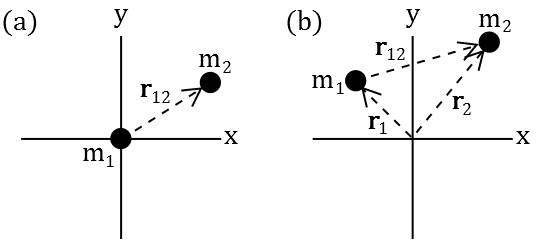
\includegraphics[width=0.6\linewidth]{Figures/2bodyproblem_coordinatesystems.png}
\caption{
Two-dimensional illustration of the three-dimensional problem of determining determining the relative distance and relative velocity between two bodies. 
In (a) body 1 with mass $m_1$ is considered stationary in position- and velocity-space, whilst body 2 with mass $m_2$ moves relative to body 1.
In (b) both body 1 and 2 moves relative to the frame of reference in position and time, yielding that the position vector between body 1 and 2 is given as $\v{r}_{12} = \v{r}_2 - \v{r}_1$.
}
\label{fig:2bodyproblem_coordinatesystems}
\end{figure}
In the codes presented in this section, solving the problem in coordinate system (a) will first be considered for simplicity. Thereafter, the codes will be extended to include the movement of body 1 relative to the coordinate system, since this will be useful when extending the codes to an N body system.  

In the problem, $\v{r}(t)$ is the three-dimensional space vector consisting of the coordinated $(x(t),y(t),z(t))$, whilst $\v{v}(t)$ is the three-dimensional velocity vector with coordinates $(v_x(t),v_y(t),v_z(t))$, both of which are dependent on time. 

In general, the considered differential equation is
\begin{align}
	\frac{dy}{dt} = f(t,y)
	\label{eq:diffEq1}
\end{align}
Which yields that
\begin{align}
	y(t) = \int f(t,y) dt
\end{align}
\fxnote{do we need to write $y_{i+1}$ eq from p. 250 in lecture notes??}
For the two bodies in a three dimensional Newtonian gravitational field this corresponds to six coupled differential equations given by the vector equations
\begin{align}
	\frac{d\v{r}}{dt} = \v{v}
	\qquad \text{and} \qquad
	\frac{d\v{v}}{dt} = - \frac{G M_1 M_2}{r^3} \v{r}
	\label{eq:diffEq2}
\end{align}
\fxnote{maybe we should divide by mass as on p. 248??}
in which $M_1$ and $M_2$ \fxnote{fix the this with $M_1$ and $M_2$} are the masses of the two bodies, respectively, whilst $r$ is the distance between the bodies.
The equations in \eqref{eq:diffEq2} are computed by the script given below in which $drdt$ corresponds to the derivative of the coordinates of the position, and $dvdt$ corresponds to the derivative of the velocity coordinates. 
\begin{lstlisting}
void Derivative(double r[3], double v[3], double (&drdt)[3], double (&dvdt)[3], double G, double mass){
    drdt[0] = v[0];
    drdt[1] = v[1];
    drdt[2] = v[2];
    double distance_squared = r[0]*r[0] + r[1]*r[1] + r[2]*r[2];
    double newtonian_force = -G*mass/pow(distance_squared,1.5);
    dvdt[0] = newtonian_force*r[0];
    dvdt[1] = newtonian_force*r[1];
    dvdt[2] = newtonian_force*r[2];
}
\end{lstlisting}
When including movement of both bodies relative to the frame of reference, the \textit{Derivative} function must be slightly modified, since then the relative position of the two bodies will be given as $\v{r}_{12} = \v{r}_2 - \v{r}_1$.
For a general case with $N$ particles, the \textit{distance\_ squared} between body $i$ and $j$, and the acceleration in $x$, $y$ and $z$ due to the Newtonian force between body $i$ and $j$ can be determined by the following lines of code.
\begin{lstlisting}
for (int j=0; j<number_of_particles; j++)
    {
        if (j!=i)
        {
            distance_squared = 0;
            for (int k=0; k<3; k++)
            {
                distance_squared += (r(i,k)-r(j,k))*(r(i,k)-r(j,k));
            }
            force_between_particles = m(j) * pow(distance_squared,-1.5);
            acc_x += G*force_between_particles*(r(j,0)-r(i,0));
            acc_y += G*force_between_particles*(r(j,1)-r(i,1));
            acc_z += G*force_between_particles*(r(j,2)-r(i,2));
        }
    }
\end{lstlisting}
The if statement in the for loop over all bodies adds up the acceleration in all three dimensions of all particles due to the presence of other particles.
Hence, for the two body problem, the argument in the if statement will only be true once for each of the two particles.